%----------------------------------------------------------------------------------------
% Parallel count sort
%----------------------------------------------------------------------------------------

\section{Parallel Count Sort using OpenMP}

\subsection{If we attempt to parallelize the \emph{for} i loop (the outer loop),
which variables should be private and which should be shared?}

The variables \emph{temp, a} should be shared and, \emph{i, j, count} should
be private.

\subsection{Parallelize the code using OpenMP directives to modify the 
Count\_sort\_parallel subroutine}

\vspace{0.5cm}
\lstinputlisting[
	style=CStyle,
	firstline=167, % First line of code
	lastline=191, % Lastl ine of code
	caption=Parallizing the code for multi-threaded execution (line 167-191 in lab3part3.c), % Caption above the listing
	label=lst:lab3part3a, % Label for referencing this listing
	frame=single, % Frame around the code listing
	showstringspaces=false, % Don't put marks in string spaces
	numbers=left, % Line numbers on left
	numberstyle=\normalsize % Line numbers styling
    ]{../code/lab3part4.c}
    

\subsection{Tabuate the speedup and efficiency for 1,2,4,8 threads and n=1000
elements}

\begin{center}
\begin{tabular}{|| c | c | c | c ||}
	\hline
	Threads & Time (s) & Speedup & Efficiency (\%) \\ [0.5ex]
	\hline 
	1 & 0.459 & N/A & 100 \\
	2 & 0.229 & 1.899 & 94.95 \\
	4 & 0.132 & 3.266 & 81.65 \\
	8 & 0.075 & 5.764 & 72.05 \\
	\hline
\end{tabular}
\end{center}

\begin{figure}[ht]
	\centering
	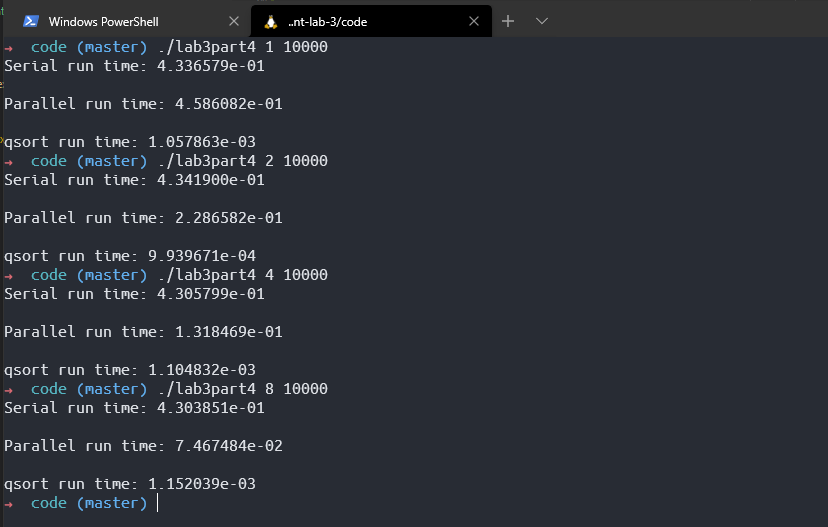
\includegraphics[width=\textwidth]{graphics/P4_b_terminal_output.PNG}
    \caption{Terminal output for execution with 1, 2, 4, 8 threads respectively
    and n=10000}
	\label{fig:lab3part4b}
\end{figure}

\subsubsection{How does the performance of the parallelized code compare to the serial
version?}

The performance of the parallelize code is better than the serial version in terms of speed
as seen in the table above. However, there is a diminishing return in the speed gain vs 
the resources (threads) allocated.

\subsection{What is the complexity of serial Count\_sort? What is the complexity of
serial qsort? Does your answer match the run times generated by the programme?}

The time complexity of serial Count\_sort is O(n), and the time complexity of
serial qsort is O(nlogn). Which means theoretically, qsort should be slower than
serial Count\_sort, however, this is not the case when looking at the run times
generated by the program in \cref{fig:lab3part4b}.